
\FloatBarrier

\raggedbottom
\subsection{Fault Localization}
\label{appendix:fault-localisation}
This section presents the descriptive results of the fault localization
part of the developer survey. Six respondents completed the fault
localization questions ($n=6$). Four additional survey participants did
not provide responses to this section. Unless stated otherwise, all
results in this subsection refer to these six respondents.

\begin{figure}[H]
    \centering
    \scriptsize
    \begin{minipage}[t]{0.47\textwidth}
        \centering
        \textbf{\scriptsize
        What percentage of your overall time do you spend
        localizing faults?}
        \vspace{0.1em}
        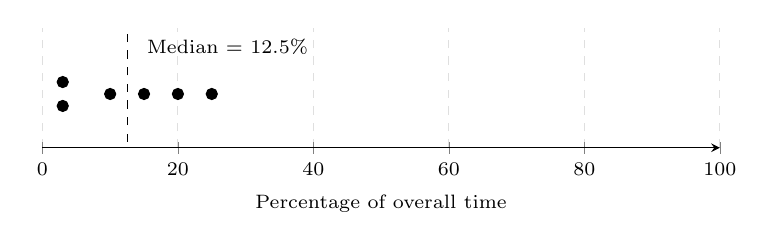
\begin{tikzpicture}
            \begin{axis}[
                width=0.84\linewidth,
                height=3.1cm,
                xmin=0,
                xmax=100,
                ymin=0.82,
                ymax=1.22,
                xtick={0,20,40,60,80,100},
                xlabel={Percentage of overall time},
                xlabel style={font=\scriptsize},
                tick label style={font=\scriptsize},
                ytick=\empty,
                axis y line=none,
                axis x line=bottom,
                grid=major,
                grid style={dashed,gray!25},
                clip=false
            ]
            \addplot[
                only marks,
                mark=*,
                mark size=2pt
            ] coordinates {
                (3,0.96)
                (3,1.04)
                (10,1.00)
                (15,1.00)
                (20,1.00)
                (25,1.00)
            };
            \draw[dashed]
                (axis cs:12.5,0.84) --
                (axis cs:12.5,1.20);
            \node[
                anchor=south west,
                font=\scriptsize
            ] at (axis cs:14,1.10)
            {Median = 12.5\%};
            \end{axis}
        \end{tikzpicture}
        \par\vspace{0.1em}
        {\scriptsize
        (a) Overall time spent localizing faults.}
    \end{minipage}\hfill
    \begin{minipage}[t]{0.47\textwidth}
        \centering
        \textbf{\scriptsize
        How long does it take to localize the fault
        of a single failure?}
        \vspace{0.1em}
        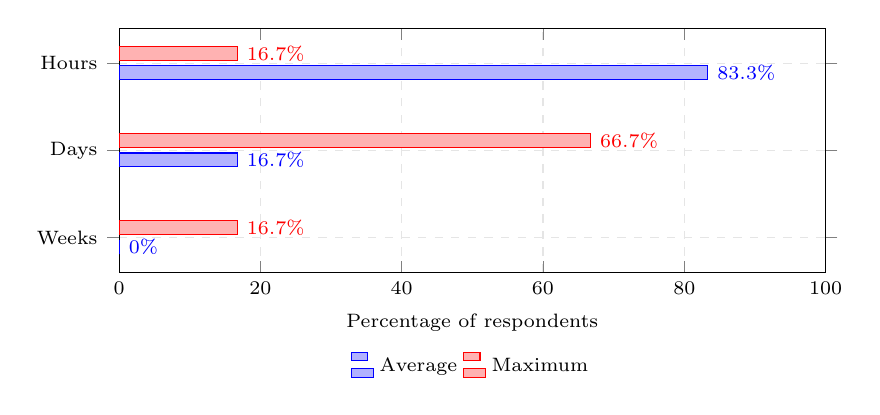
\begin{tikzpicture}
            \begin{axis}[
                xbar,
                width=0.74\linewidth,
                height=3.1cm,
                scale only axis,
                xmin=0,
                xmax=100,
                xtick={0,20,40,60,80,100},
                xlabel={Percentage of respondents},
                xlabel style={font=\scriptsize},
                symbolic y coords={
                    {Weeks},
                    {Days},
                    {Hours}
                },
                ytick=data,
                yticklabel style={font=\scriptsize},
                tick label style={font=\scriptsize},
                nodes near coords={
                    \pgfmathprintnumber[fixed,precision=1]
                    {\pgfplotspointmeta}\%
                },
                every node near coord/.append style={
                    font=\scriptsize
                },
                point meta=x,
                bar width=5pt,
                enlarge y limits=0.20,
                legend style={
                    at={(0.5,-0.30)},
                    anchor=north,
                    legend columns=2,
                    font=\scriptsize,
                    draw=none
                },
                grid=major,
                grid style={dashed,gray!20}
            ]
            % Average localization time
            \addplot coordinates {
                (0,{Weeks})
                (16.7,{Days})
                (83.3,{Hours})
            };
            % Maximum localization time
            \addplot coordinates {
                (16.7,{Weeks})
                (66.7,{Days})
                (16.7,{Hours})
            };
            \legend{
                Average,
                Maximum
            }
            \end{axis}
        \end{tikzpicture}
        \par\vspace{0.1em}
        {\scriptsize
        (b) Average and maximum localization time.}
    \end{minipage}
    \caption{Reported effort and duration of fault localization
    activities ($n=6$).}
    \label{fig:appendix-fault-localization-time}
\end{figure}

\vspace{-0.6em}

\begin{figure}[H]
    \centering
    \textbf{\scriptsize
    How much knowledge is required for fault localization?}
    \vspace{0.15em}
    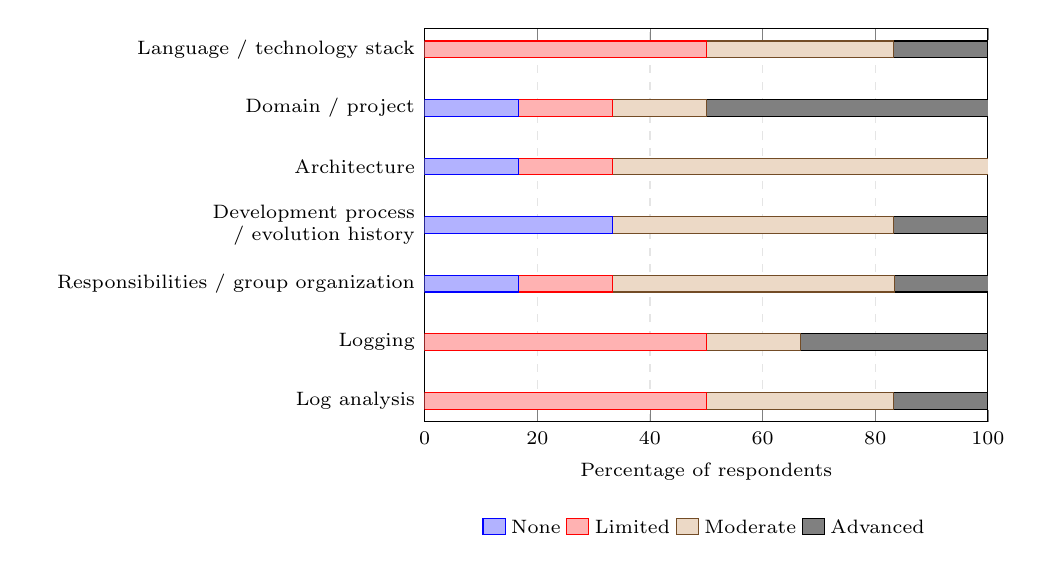
\begin{tikzpicture}
        \begin{axis}[
            xbar stacked,
            width=0.59\textwidth,
            height=5.0cm,
            scale only axis,
            xmin=0,
            xmax=100,
            xtick={0,20,40,60,80,100},
            xlabel={Percentage of respondents},
            xlabel style={font=\scriptsize},
            symbolic y coords={
                {Log analysis},
                {Logging},
                {Responsibilities / group organization},
                {Development process / evolution history},
                {Architecture},
                {Domain / project},
                {Language / technology stack}
            },
            ytick=data,
            yticklabel style={
                text width=4.8cm,
                align=right,
                font=\scriptsize
            },
            tick label style={font=\scriptsize},
            bar width=6pt,
            enlarge y limits=0.06,
            legend style={
                at={(0.5,-0.22)},
                anchor=north,
                legend columns=4,
                font=\scriptsize,
                draw=none
            },
            grid=major,
            grid style={dashed,gray!20}
        ]
        % None
        \addplot coordinates {
            (0,{Log analysis})
            (0,{Logging})
            (16.7,{Responsibilities / group organization})
            (33.3,{Development process / evolution history})
            (16.7,{Architecture})
            (16.7,{Domain / project})
            (0,{Language / technology stack})
        };
        % Limited
        \addplot coordinates {
            (50,{Log analysis})
            (50,{Logging})
            (16.7,{Responsibilities / group organization})
            (0,{Development process / evolution history})
            (16.7,{Architecture})
            (16.7,{Domain / project})
            (50,{Language / technology stack})
        };
        % Moderate
        \addplot coordinates {
            (33.3,{Log analysis})
            (16.7,{Logging})
            (50,{Responsibilities / group organization})
            (50,{Development process / evolution history})
            (66.7,{Architecture})
            (16.7,{Domain / project})
            (33.3,{Language / technology stack})
        };
        % Advanced
        \addplot coordinates {
            (16.7,{Log analysis})
            (33.3,{Logging})
            (16.7,{Responsibilities / group organization})
            (16.7,{Development process / evolution history})
            (0,{Architecture})
            (50,{Domain / project})
            (16.7,{Language / technology stack})
        };
        \legend{
            None,
            Limited,
            Moderate,
            Advanced
        }
        \end{axis}
    \end{tikzpicture}
    \caption{Reported level of knowledge required for fault localization
    across different areas ($n=6$).}
    \label{fig:appendix-fault-localization-knowledge}
\end{figure}

\begin{figure}[H]
    \centering
    \textbf{\scriptsize
    To which extent do you agree or disagree with the following
    statements?}
    \vspace{0.15em}
    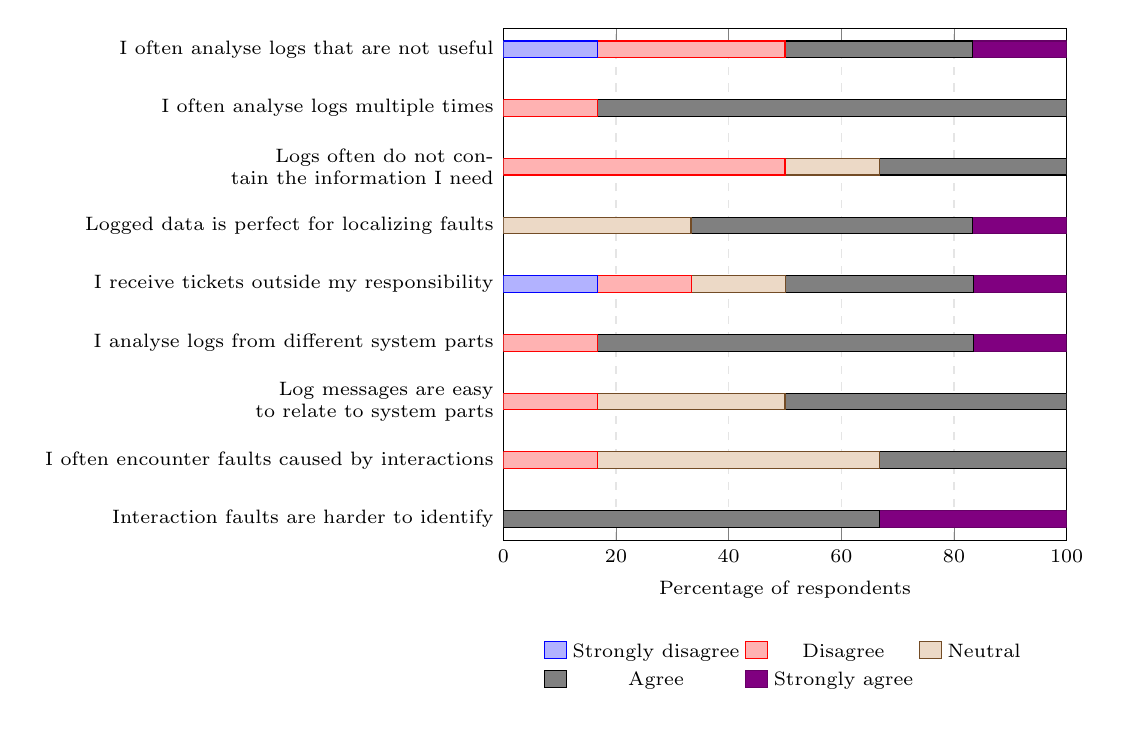
\begin{tikzpicture}
        \begin{axis}[
            xbar stacked,
            width=0.59\textwidth,
            height=6.5cm,
            scale only axis,
            xmin=0,
            xmax=100,
            xtick={0,20,40,60,80,100},
            xlabel={Percentage of respondents},
            xlabel style={font=\scriptsize},
            symbolic y coords={
                {Interaction faults are harder to identify},
                {I often encounter faults caused by interactions},
                {Log messages are easy to relate to system parts},
                {I analyse logs from different system parts},
                {I receive tickets outside my responsibility},
                {Logged data is perfect for localizing faults},
                {Logs often do not contain the information I need},
                {I often analyse logs multiple times},
                {I often analyse logs that are not useful}
            },
            ytick=data,
            yticklabel style={
                text width=5.8cm,
                align=right,
                font=\scriptsize
            },
            tick label style={font=\scriptsize},
            bar width=6pt,
            enlarge y limits=0.045,
            legend style={
                at={(0.5,-0.18)},
                anchor=north,
                legend columns=3,
                font=\scriptsize,
                draw=none
            },
            grid=major,
            grid style={dashed,gray!20}
        ]
        % Strongly disagree
        \addplot coordinates {
            (0,{Interaction faults are harder to identify})
            (0,{I often encounter faults caused by interactions})
            (0,{Log messages are easy to relate to system parts})
            (0,{I analyse logs from different system parts})
            (16.7,{I receive tickets outside my responsibility})
            (0,{Logged data is perfect for localizing faults})
            (0,{Logs often do not contain the information I need})
            (0,{I often analyse logs multiple times})
            (16.7,{I often analyse logs that are not useful})
        };
        % Disagree
        \addplot coordinates {
            (0,{Interaction faults are harder to identify})
            (16.7,{I often encounter faults caused by interactions})
            (16.7,{Log messages are easy to relate to system parts})
            (16.7,{I analyse logs from different system parts})
            (16.7,{I receive tickets outside my responsibility})
            (0,{Logged data is perfect for localizing faults})
            (50,{Logs often do not contain the information I need})
            (16.7,{I often analyse logs multiple times})
            (33.3,{I often analyse logs that are not useful})
        };
        % Neutral
        \addplot coordinates {
            (0,{Interaction faults are harder to identify})
            (50,{I often encounter faults caused by interactions})
            (33.3,{Log messages are easy to relate to system parts})
            (0,{I analyse logs from different system parts})
            (16.7,{I receive tickets outside my responsibility})
            (33.3,{Logged data is perfect for localizing faults})
            (16.7,{Logs often do not contain the information I need})
            (0,{I often analyse logs multiple times})
            (0,{I often analyse logs that are not useful})
        };
        % Agree
        \addplot coordinates {
            (66.7,{Interaction faults are harder to identify})
            (33.3,{I often encounter faults caused by interactions})
            (50,{Log messages are easy to relate to system parts})
            (66.7,{I analyse logs from different system parts})
            (33.3,{I receive tickets outside my responsibility})
            (50,{Logged data is perfect for localizing faults})
            (33.3,{Logs often do not contain the information I need})
            (83.3,{I often analyse logs multiple times})
            (33.3,{I often analyse logs that are not useful})
        };
        % Strongly agree
        \addplot coordinates {
            (33.3,{Interaction faults are harder to identify})
            (0,{I often encounter faults caused by interactions})
            (0,{Log messages are easy to relate to system parts})
            (16.7,{I analyse logs from different system parts})
            (16.7,{I receive tickets outside my responsibility})
            (16.7,{Logged data is perfect for localizing faults})
            (0,{Logs often do not contain the information I need})
            (0,{I often analyse logs multiple times})
            (16.7,{I often analyse logs that are not useful})
        };
        \legend{
            Strongly disagree,
            Disagree,
            Neutral,
            Agree,
            Strongly agree
        }
        \end{axis}
    \end{tikzpicture}
    \caption{Respondents' perceptions and experiences concerning fault
    localization ($n=6$). Statement labels were shortened for
    readability.}
    \label{fig:appendix-fault-localization-likert}
\end{figure}

\FloatBarrier
\subsubsection{Open-Ended Fault Localization Responses}
\label{appendix:open-ended-fault-localization}
{\footnotesize
The following tables present lightly paraphrased versions of the
open-ended survey responses. The responses were rephrased for
readability and conciseness while preserving their original meaning.
No additional thematic coding was applied.
}

\begingroup
\scriptsize
\renewcommand{\arraystretch}{0.90}
\setlength{\tabcolsep}{3pt}
\begin{longtable}{
    @{}
    >{\centering\arraybackslash}p{0.04\textwidth}
    >{\RaggedRight\arraybackslash}p{0.43\textwidth}
    >{\RaggedRight\arraybackslash}p{0.46\textwidth}
    @{}
}

\\\\
\toprule
\textbf{ID} &
\textbf{How do you identify the functionality or part of the system affected by a log message?} &
\textbf{What data are used in addition to logs?} \\\\
\midrule
\endfirsthead
\multicolumn{3}{l}{
    \scriptsize\textit{Table continued from previous page}
}
\\\\[0.1em]
\toprule
\textbf{ID} &
\textbf{How do you identify the functionality or part of the system affected by a log message?} &
\textbf{What data are used in addition to logs?} \\\\
\midrule
\endhead
\midrule
\multicolumn{3}{r}{
    \scriptsize\textit{Continued on next page}
}
\\\\
\endfoot
\bottomrule
\endlastfoot

P1 &
The cause of the problem is investigated and traced back to the main
underlying problem so that similar or future errors can also be
addressed. &
Debugger information and variable values from different program states
are used.
\\\\[0.1em]

P2 &
Semi-structured log messages containing the corresponding class name
are used to identify the affected part of the system. &
System configuration exports are used as additional information.
\\\\[0.1em]

P3 &
The affected functionality is identified directly from the log or its
origin information where possible. Otherwise, the source code is
searched. &
Files produced by the system may be inspected when relevant.
\\\\[0.1em]

P4 &
The affected part of the system is identified using labels associated
with the log entries. &
Database entries are used as additional information.
\\\\[0.1em]

P5 &
Installer logs containing WiX Toolset-specific messages are used to
identify the affected functionality. &
No additional data were reported.
\\\\[0.1em]

P6 &
Unexpected or missing input or output data are used to identify the
affected part of the system. &
Clients are asked to describe the error and, where possible, provide
a video demonstrating the problem.
\\\\
\caption{Paraphrased responses concerning identification of affected
system functionality and additional data used for fault localization.}
\label{tab:appendix-fault-identification}
\end{longtable}
\endgroup

\vspace{-0.4em}
\begingroup
\scriptsize
\renewcommand{\arraystretch}{0.90}
\setlength{\tabcolsep}{3pt}
\begin{longtable}{
    @{}
    >{\centering\arraybackslash}p{0.035\textwidth}
    >{\RaggedRight\arraybackslash}p{0.27\textwidth}
    >{\RaggedRight\arraybackslash}p{0.25\textwidth}
    >{\RaggedRight\arraybackslash}p{0.34\textwidth}
    @{}
}

\\\\
\toprule
\textbf{ID} &
\textbf{Identifying interactions} &
\textbf{Handling interaction failures} &
\textbf{Example} \\\\
\midrule
\endfirsthead
\multicolumn{4}{l}{
    \scriptsize\textit{Table continued from previous page}
}
\\\\[0.1em]
\toprule
\textbf{ID} &
\textbf{Identifying interactions} &
\textbf{Handling interaction failures} &
\textbf{Example} \\\\
\midrule
\endhead
\midrule
\multicolumn{4}{r}{
    \scriptsize\textit{Continued on next page}
}
\\\\
\endfoot
\bottomrule
\endlastfoot

P1 &
The error is traced backwards until the main underlying problem is
found. &
Failures are listed, the developer responsible for the relevant
implementation is identified, and the error is then investigated and
fixed. &
Rather than providing a specific failure example, the response
described a process of detecting the error, contacting the relevant
developer, and either collaboratively or independently fixing it.
\\\\[0.1em]

P2 &
No clear response was provided. &
The owners of the affected system parts are contacted. &
An example involved business logic communicating with a third-party
system through an adapter.
\\\\[0.1em]

P3 &
A thorough understanding of how the system operates is developed. &
The involved functionalities are isolated, analysed individually, and
then analysed together. &
No specific example was provided.
\\\\[0.1em]

P4 &
Historically accumulated company knowledge is used to understand
interactions between system components. &
The approach depends on the particular failure. &
An example involved application functionality that depended on
mandatory hardware components.
\\\\[0.1em]

P5 &
No response was provided. &
No response was provided. &
No response was provided.
\\\\[0.1em]

P6 &
The normal behaviour of the individual functionalities is considered
and their overall interaction is examined. &
The people responsible for the other functionalities or systems are
contacted and the problem is investigated collaboratively. &
Two interacting systems exchanged control signals. A required signal
was either not received or occurred with problematic timing. The
analysis therefore had to determine whether the fault originated in
another team's system or from timing and latency between the systems.
\\\\
\caption{Paraphrased responses concerning failures involving
interactions between multiple functionalities or system parts.}
\label{tab:appendix-fault-interactions}
\end{longtable}
\endgroup

\clearpage
\vspace{-0.4em}
\begingroup
\scriptsize
\renewcommand{\arraystretch}{0.90}
\setlength{\tabcolsep}{3pt}
\begin{longtable}{
    @{}
    >{\centering\arraybackslash}p{0.035\textwidth}
    >{\RaggedRight\arraybackslash}p{0.29\textwidth}
    >{\RaggedRight\arraybackslash}p{0.29\textwidth}
    >{\RaggedRight\arraybackslash}p{0.30\textwidth}
    @{}
}

\\\\
\toprule
\textbf{ID} &
\textbf{Colleague involvement} &
\textbf{Challenges} &
\textbf{Recommended practices} \\\\
\midrule
\endfirsthead
\multicolumn{4}{l}{
    \scriptsize\textit{Table continued from previous page}
}
\\\\[0.1em]
\toprule
\textbf{ID} &
\textbf{Colleague involvement} &
\textbf{Challenges} &
\textbf{Recommended practices} \\\\
\midrule
\endhead
\midrule
\multicolumn{4}{r}{
    \scriptsize\textit{Continued on next page}
}
\\\\
\endfoot
\bottomrule
\endlastfoot

P1 &
The extent of colleague involvement depends on how strongly colleagues
were involved in the relevant project and implementation. &
Finding the correct location of a fault in a large project can be
difficult. &
Trace the error backwards until the underlying root problem is found.
\\\\[0.1em]

P2 &
Colleagues support confirmation of the issue from the logs and help
define an appropriate solution or fix. &
No specific challenge was reported. &
No specific strategy was reported.
\\\\[0.1em]

P3 &
When software belonging to colleagues is involved in the problem,
fault localization becomes a collaborative process similar to pair
programming. &
The main difficulty arises when the respondent is unfamiliar with how
a system works. &
First obtain an overview of the system structure and its logging
practices or policies.
\\\\[0.1em]

P4 &
Developers inspect the logs associated with the parts of the system
for which they are responsible. &
A lack of historically accumulated company knowledge makes fault
localization more difficult. &
Use text search to locate relevant information.
\\\\[0.1em]

P5 &
No specific colleague involvement was reported. &
No specific challenge was reported. &
No specific strategy was reported.
\\\\[0.1em]

P6 &
The behaviour of the overall system is discussed collaboratively to
identify the source of the fault. &
Timing and latency across multiple systems are difficult to analyse,
particularly when other systems have changed without notification. &
Discuss the expected behaviour of all involved systems, construct a
flowchart of their interactions, and compare the expected sequence
with the observed behaviour.
\\\\
\caption{Paraphrased responses concerning collaboration, challenges,
and recommended practices for fault localization.}
\label{tab:appendix-fault-practices}
\end{longtable}
\endgroup


\FloatBarrier
\clearpage
\flushbottom
